\documentclass[10pt,a4paper]{article}

\usepackage[T1]{fontenc}
\usepackage[utf8]{inputenc}
\usepackage[english]{babel}
\usepackage{geometry}
\geometry{top=2.2cm,bottom=2.3cm,left=2.2cm,right=2.2cm}

\usepackage{amsmath,amssymb,bm}
\setcounter{MaxMatrixCols}{20}
\usepackage{graphicx}
\usepackage{xcolor}
\usepackage{tcolorbox}
\tcbuselibrary{skins,breakable}
\usepackage{booktabs}
\usepackage{fancyhdr}
\usepackage{caption}
\usepackage{float}
\usepackage{listings}
\usepackage{tikz}
\usetikzlibrary{arrows.meta,positioning,calc}
\usepackage[hidelinks]{hyperref}

% ---------------------------------------------------------- metadata ---
\newcommand{\Institution}{Instituto Superior Técnico}
\newcommand{\Programme}{MEAer}
\newcommand{\CourseTitle}{Unmanned Aerial Vehicles}
\newcommand{\ReportTitle}{Estimation of Motion Variables of the Parrot AR.Drone}
\newcommand{\LabNumber}{2}
\newcommand{\Semester}{2026/2027 -- First Semester}
\newcommand{\GroupNumber}{17}            % TODO: group number
\newcommand{\Instructor}{Prof.\ David Cabecinhas}

% name / number / (one line per author)
\newcommand{\AuthorList}{%
  \AuthorRow{IST1116311}{Caio Hokama Freitas}%
  \AuthorRow{IST1113325}{Majid Attarzadeh}%   TODO: real IST number
}

% ------------------------------------------------------------ colours ---
\definecolor{istblue}{HTML}{03ABE6}
\definecolor{qfill}{HTML}{E4F6FD}
\definecolor{qtitle}{HTML}{0288B0}
\definecolor{greyfill}{HTML}{F7F7F7}
\definecolor{greyline}{HTML}{D9D9D9}
\definecolor{tagT}{HTML}{B45309}
\definecolor{tagL}{HTML}{2E7D32}

% ------------------------------------------------- header and footer ---
\pagestyle{fancy}
\fancyhf{}
\fancyhead[L]{\footnotesize IST}
\fancyhead[R]{\footnotesize ULisboa}
\fancyfoot[C]{\footnotesize\thepage}
\renewcommand{\headrulewidth}{0.6pt}
\renewcommand{\footrulewidth}{0.4pt}

% ------------------------------------------- question / answer boxes ---
% #1 is T or L; the colours are named tagT and tagL.
\newcommand{\tagpill}[1]{%
  \begingroup
  \setlength{\fboxsep}{2pt}%
  \colorbox{tag#1}{\textcolor{white}{\scriptsize\bfseries~#1~}}%
  \endgroup}

% \tagpills{T}, \tagpills{L}, \tagpills{T+L} or \tagpills{T + L}: one pill per tag, joined by "+".
\makeatletter
\newcommand{\tagpills}[1]{%
  \edef\tagpills@list{\zap@space#1 \@empty}%
  \expandafter\tagpills@next\tagpills@list+\@nil}
\def\tagpills@next#1+#2\@nil{%
  \tagpill{#1}%
  \ifx\relax#2\relax\else
    \hspace{3pt}{\small\bfseries\textcolor{qtitle}{+}}\hspace{3pt}%
    \tagpills@next#2\@nil
  \fi}
\makeatother

% \begin{question}{2.1}{T}  ... \end{question}
\newenvironment{question}[2]{%
  \begin{tcolorbox}[breakable,enhanced,colback=qfill,colframe=qfill,
    borderline west={3pt}{0pt}{istblue},boxrule=0pt,arc=2pt,
    left=8pt,right=8pt,top=7pt,bottom=7pt,before skip=12pt,after skip=6pt]
  \textcolor{qtitle}{\bfseries Question #1}\hspace{4pt}\tagpills{#2}\par\vspace{3pt}%
}{\end{tcolorbox}}

\newenvironment{answer}{%
  \begin{tcolorbox}[breakable,enhanced,colback=white,colframe=greyline,
    boxrule=0.6pt,arc=2pt,left=8pt,right=8pt,top=7pt,bottom=7pt,
    before skip=0pt,after skip=12pt]
}{\end{tcolorbox}}

\newcommand{\todoanswer}{\emph{Write your answer here.}}

% ----------------------------------------------------- code listings ---
\lstdefinestyle{mat}{
  language=Matlab, basicstyle=\ttfamily\footnotesize,
  keywordstyle=\color{blue!60!black}, commentstyle=\color{green!40!black},
  stringstyle=\color{purple}, numbers=none, frame=single,
  rulecolor=\color{greyline}, backgroundcolor=\color{greyfill},
  breaklines=true, showstringspaces=false, columns=fullflexible,
}
\lstset{style=mat}

% --------------------------------------------------------- shortcuts ---
\newcommand{\R}{\mathbb{R}}
\newcommand{\fB}{\{B\}}
\newcommand{\fI}{\{I\}}
\newcommand{\Bp}{{}^{B}\bm{p}}

\captionsetup{font=small,labelfont=bf}

% =======================================================================
\begin{document}

% ------------------------------------------------------- cover page ---
\newcommand{\AuthorRow}[2]{%
  \makebox[3.2cm][l]{\textbf{N.\textsuperscript{o}: #1}}%
  \makebox[8.2cm][l]{\textbf{Name: #2}}%
  \textbf{Signature:}\\[1.4ex]}

\begin{titlepage}
\thispagestyle{empty}
\noindent
\includegraphics[width=3.2cm]{figs/ist_logo.png}

\vspace{1.6cm}
\begin{center}
  {\large \Institution}\\[1.0em]
  {\large \Programme}\\[2.4em]
  {\LARGE \bfseries \CourseTitle}\\[1.2em]
  {\normalsize \Semester}

  \vspace{4.2cm}

  {\LARGE \underline{Laboratory \LabNumber}}\\[0.8em]
  {\small \itshape \ReportTitle}\\[1.8em]
  {\normalsize \bfseries \underline{Group \GroupNumber}}
\end{center}

\vspace{1.4em}
\noindent\AuthorList

\vfill
\begin{center}
  {\normalsize \underline{Instructor: \Instructor}}
\end{center}
\vspace{2.2cm}
\end{titlepage}

\setcounter{page}{1}
\setcounter{section}{2}   % the guide's Section 1 (Introduction) is not reproduced

% =====================================================================
\section{Modeling and characterization of the sensors}

% ------------------------------------------------------------ Q3.1 ---
\begin{question}{3.1}{L}
    Characterize the accelerometers and rate gyro disturbances that are present on the measurements, by computing the mean and covariance of the measurements obtained in \emph{Experiment A}.
\end{question}

\begin{answer}
In Experiment A, the drone was kept stationary on the ground
with its motors switched off. The accelerometer and gyroscope
measurements were analyzed to characterize the sensor disturbances.

The sample mean was computed as
\[
\boldsymbol{\mu} =
\frac{1}{N}\sum_{k=1}^{N}\mathbf{x}_k,
\]
and the sample covariance matrix was calculated as
\[
\boldsymbol{\Sigma} =
\frac{1}{N-1}
\sum_{k=1}^{N}
(\mathbf{x}_k-\boldsymbol{\mu})
(\mathbf{x}_k-\boldsymbol{\mu})^T.
\]

\paragraph{Accelerometer}
The estimated mean accelerometer measurement is
\[
\boldsymbol{\mu}_{a,A} =
\begin{bmatrix}
8.4\\
-40.5\\
-1011.6
\end{bmatrix}.
\]
The corresponding covariance matrix is
\[
\boldsymbol{\Sigma}_{a,A} =
\begin{bmatrix}
56.7 & 34.3 & 8.4\\
34.3 & 32.9 & 86.5\\
8.4 & 86.5 & 1728.6
\end{bmatrix}.
\]
The standard deviations are
\[
\boldsymbol{\sigma}_{a,A} =
\begin{bmatrix}
7.5272 & 5.7385 & 41.5767
\end{bmatrix}.
\]
The acceleration magnitude was approximately \(1012.4\)
units. Since the drone was stationary, this measurement is
mainly associated with gravity. The magnitude suggests a
scale of approximately \(1000\) units per \(g\), although
the exact measurement units were not specified in the
signal metadata.

\paragraph{Gyroscope}
The estimated mean gyroscope measurement is
\[
\boldsymbol{\mu}_{g,A} =
\begin{bmatrix}
0.0561\\
-0.0896\\
0.0030
\end{bmatrix}.
\]
The covariance matrix is
\[
\boldsymbol{\Sigma}_{g,A} =
\begin{bmatrix}
0.0019 & -0.0001 & 0\\
-0.0001 & 0.0019 & 0\\
0 & 0 & 0.0015
\end{bmatrix}.
\]
The standard deviations are
\[
\boldsymbol{\sigma}_{g,A} =
\begin{bmatrix}
0.0440 & 0.0430 & 0.0390
\end{bmatrix}.
\]
Ideally, the gyroscope measurements should be zero when
the drone is stationary. The small non-zero mean values
indicate possible sensor bias, while the covariance matrix
describes the measurement variability and noise.

Overall, Experiment A provides a baseline characterization
of the sensor disturbances in the absence of motor-induced
vibrations.
\end{answer}

% ------------------------------------------------------------ Q3.2 ---
\begin{question}{3.2}{L}
    Repeat the previous computations for \emph{Experiment B}. Discuss the new sources of disturbances leading to the increase of uncertainty on the measurements.
\end{question}

\begin{answer}
The mean and covariance of the accelerometer and gyroscope measurements were calculated using the data collected in Experiment B. The sample mean is given by
\[
\boldsymbol{\mu}=\frac{1}{N}\sum_{k=1}^{N}\mathbf{x}_k
\]
and the sample covariance matrix is
\[
\boldsymbol{\Sigma}=
\frac{1}{N-1}\sum_{k=1}^{N}
(\mathbf{x}_k-\boldsymbol{\mu})
(\mathbf{x}_k-\boldsymbol{\mu})^T.
\]

\paragraph{Accelerometer}
The mean accelerometer measurement is
\[
\boldsymbol{\mu}_{a,B}=
\begin{bmatrix}
44.7\\
67.1\\
-1005.7
\end{bmatrix}.
\]
The covariance matrix is
\[
\boldsymbol{\Sigma}_{a,B}=
\begin{bmatrix}
340 & 698 & -46\\
698 & 10934 & 157\\
-46 & 157 & 820
\end{bmatrix}.
\]
The corresponding standard deviations are
\[
\boldsymbol{\sigma}_{a,B}=
\begin{bmatrix}
18.4315\\
104.5678\\
28.6408
\end{bmatrix}.
\]

\paragraph{Gyroscope}
The mean gyroscope measurement is
\[
\boldsymbol{\mu}_{g,B}=
\begin{bmatrix}
-0.2643\\
0.1609\\
-0.3239
\end{bmatrix}.
\]
The covariance matrix is
\[
\boldsymbol{\Sigma}_{g,B}=
\begin{bmatrix}
34.8604 & 4.5753 & 18.1459\\
4.5753 & 7.9967 & 8.9292\\
18.1459 & 8.9292 & 34.6251
\end{bmatrix}.
\]
The corresponding standard deviations are
\[
\boldsymbol{\sigma}_{g,B}=
\begin{bmatrix}
5.9043\\
2.8278\\
5.8843
\end{bmatrix}.
\]

Compared with Experiment A, the uncertainty in the measurements increases considerably when the motors are running. This is particularly evident in the accelerometer \(y\)-axis and in all three gyroscope axes. The accelerometer standard deviation along the \(y\)-axis increases from approximately \(5.74\) to \(104.57\), while the gyroscope standard deviations also increase substantially.

The main additional disturbance source is the mechanical vibration generated by the motors and propellers. These vibrations are transmitted through the drone frame to the IMU, affecting both the accelerometer and gyroscope measurements. Motor rotation and propeller imbalance may also introduce periodic disturbances.

It should be noted that not all accelerometer axes show an increase in standard deviation. In particular, the standard deviation along the \(z\)-axis is lower than in Experiment A. Therefore, the effect of motor vibration is not identical in every direction.

Overall, Experiment B demonstrates that operating the motors introduces significant additional disturbances. The calculated covariance matrices represent the total measurement variability, including sensor noise and motor-induced vibrations, rather than the intrinsic sensor noise alone.
\end{answer}

% ------------------------------------------------------------ Q3.3 ---
\begin{question}{3.3}{L}
    Repeat the previous computations for \emph{Experiment C}. Discuss the new sources of disturbances leading to the increase of uncertainty on the measurements.
\end{question}

\begin{answer}
The mean and covariance of the accelerometer and gyroscope measurements were calculated using the data collected in Experiment C.

The sample mean is calculated as
\[
\boldsymbol{\mu}=\frac{1}{N}\sum_{k=1}^{N}\mathbf{x}_k
\]
and the sample covariance matrix is
\[
\boldsymbol{\Sigma}=
\frac{1}{N-1}\sum_{k=1}^{N}
(\mathbf{x}_k-\boldsymbol{\mu})
(\mathbf{x}_k-\boldsymbol{\mu})^T.
\]

\paragraph{Accelerometer}
The mean accelerometer measurement is
\[
\boldsymbol{\mu}_{a,C}=
\begin{bmatrix}
9.0\\
-41.6\\
-1005.8
\end{bmatrix}.
\]
The covariance matrix is
\[
\boldsymbol{\Sigma}_{a,C}=
\begin{bmatrix}
712.4 & -143.5 & -1416.7\\
-143.5 & 139.4 & 535.8\\
-1416.7 & 535.8 & 8128.0
\end{bmatrix}.
\]
The corresponding standard deviations are
\[
\boldsymbol{\sigma}_{a,C}=
\begin{bmatrix}
26.6915\\
11.8067\\
90.1554
\end{bmatrix}.
\]

\paragraph{Gyroscope}
The mean gyroscope measurement is
\[
\boldsymbol{\mu}_{g,C}=
\begin{bmatrix}
0.0637\\
-0.0140\\
-0.0319
\end{bmatrix}.
\]
The covariance matrix is
\[
\boldsymbol{\Sigma}_{g,C}=
\begin{bmatrix}
12.4605 & 6.3025 & 1.9930\\
6.3025 & 18.2419 & 2.5171\\
1.9930 & 2.5171 & 4.5785
\end{bmatrix}.
\]
The corresponding standard deviations are
\[
\boldsymbol{\sigma}_{g,C}=
\begin{bmatrix}
3.5299\\
4.2711\\
2.1397
\end{bmatrix}.
\]

Compared with Experiment A, the measurements in Experiment C show considerably higher variability. The accelerometer standard deviations increase in all three axes, particularly along the \(z\)-axis, where the standard deviation reaches approximately \(90.16\). The gyroscope standard deviations also increase significantly.

In addition to motor and propeller vibrations, several disturbance sources are present during hovering flight. These include small attitude variations, translational movements, altitude corrections, and continuous control actions performed by the flight controller to maintain the hovering position. External disturbances, such as air currents, may also affect the drone.

The accelerometer measures both gravitational acceleration and the drone's actual linear acceleration. Consequently, during flight, its measurements do not represent gravity alone. This contributes to the increased variability observed in the accelerometer data.

The covariance matrices therefore describe the combined effects of sensor noise, mechanical vibrations, and actual drone motion. They should not be interpreted as measurements of intrinsic sensor noise alone.
\end{answer}

% ------------------------------------------------------------ Q3.4 ---
\begin{question}{3.4}{L}
   To later evaluate filtering effects, compute the pitch and roll inclinometer data from the accelerometer measurements, and identify these estimates as raw pitch and roll measurements. Comment the results.
\end{question}

\begin{answer}
\paragraph{Computation of pitch and roll from accelerometer measurements}
The pitch and roll angles can be estimated from the accelerometer measurements by assuming that the measured acceleration is mainly due to gravity.

Since the accelerometer \(z\)-axis measurement is negative when the drone is at rest, the following expressions are used:
\[
\theta_{\mathrm{raw}} =
\operatorname{atan2}
\left(
-a_x,\sqrt{a_y^2+a_z^2}
\right)
\]
\[
\phi_{\mathrm{raw}} =
\operatorname{atan2}(a_y,-a_z)
\]
where \(a_x\), \(a_y\), and \(a_z\) are the accelerometer measurements. The resulting angles are converted from radians to degrees:
\[
\theta_{\mathrm{deg}}=
\theta_{\mathrm{raw}}\frac{180}{\pi}
\]
\[
\phi_{\mathrm{deg}}=
\phi_{\mathrm{raw}}\frac{180}{\pi}.
\]

The following MATLAB code was used to calculate the angles for each experiment:

\begin{lstlisting}
% Experiment A
pitchA = rad2deg(atan2(-accA(:,1), ...
    sqrt(accA(:,2).^2 + accA(:,3).^2)));

rollA = rad2deg(atan2(accA(:,2), -accA(:,3)));

% Experiment B
pitchB = rad2deg(atan2(-accB(:,1), ...
    sqrt(accB(:,2).^2 + accB(:,3).^2)));

rollB = rad2deg(atan2(accB(:,2), -accB(:,3)));

% Experiment C
pitchC = rad2deg(atan2(-accC(:,1), ...
    sqrt(accC(:,2).^2 + accC(:,3).^2)));

rollC = rad2deg(atan2(accC(:,2), -accC(:,3)));

% Calculate mean and standard deviation
mean_pitch = [mean(pitchA), mean(pitchB), mean(pitchC)];
std_pitch  = [std(pitchA), std(pitchB), std(pitchC)];

mean_roll = [mean(rollA), mean(rollB), mean(rollC)];
std_roll  = [std(rollA), std(rollB), std(rollC)];
\end{lstlisting}

\paragraph{Results}
The calculated mean and standard deviation of the raw pitch and roll angles are summarized below.

\begin{center}
\begin{tabular}{@{}lrrrr@{}}
\toprule
Experiment & Mean Pitch (deg) & Std.\ Pitch (deg) & Mean Roll (deg) & Std.\ Roll (deg) \\
\midrule
A & $-0.4741$ & $0.4251$ & $-2.2888$ & $0.3155$ \\
B & $-2.5190$ & $1.0263$ & $3.7619$  & $5.7742$ \\
C & $-0.4598$ & $1.6120$ & $-2$      & \\
\bottomrule
\end{tabular}
\end{center}
\end{answer}

% =====================================================================
\section{Kalman filters}

% ------------------------------------------------------------ Q4.1 ---
\begin{question}{4.1}{T + L}
 Design, implement, and evaluate a steady-state Kalman filter for pitch estimation
based on measurements of the pitch inclinometer and on rate gyro measurement $\omega_{ym}$. To tackle the filter gain computation you can use kalman() or estim() Matlab commands.
\end{question}

\begin{answer}
In a Kalman filter the rate gyro is treated as a known
\emph{input} (it measures the derivative of the angle), and the
inclinometer as the \emph{output} (it measures the angle itself).
For small angles, $\dot\theta\approx q$ and $\dot\phi\approx p$, so for
pitch
\[
  \dot\theta=\omega_{y_m}+w_\theta,\qquad
  y_\theta=\theta+v_\theta ,
\]
and for roll
\[
  \dot\phi=\omega_{x_m}+w_\phi,\qquad
  y_\phi=\phi+v_\phi ,
\]
where $y_\theta\equiv\theta_m$ and $y_\phi\equiv\phi_m$ are the
inclinometer readings. $w$ is the gyro noise (process noise) and $v$ the
inclinometer noise (measurement noise), both assumed zero-mean, white and
independent.

The standard Kalman filter is
\[
\begin{aligned}
&\dot{x} = Ax + Bu + w\\
&y = Cx + v\\
&\dot{\hat{x}} = A\hat{x} + Bu + L(y - C\hat{x})
\end{aligned}
\]

The two equations are independent so we can combine both angles as
$\mathbf{x} = [\phi \quad \theta]^T$, $\mathbf{y} = [\phi_m \quad \theta_m]^T$,
$\mathbf{u} = [\omega_{x_m} \quad \omega_{y_m}]^T$, $A = \mathbf{0}$,
$B = C = I_2$, which gives the filter implemented
\[
\begin{aligned}
&\dot{x} = u + w\\
&y = x + v\\
&\dot{\hat{x}} = u + L(y - \hat{x})
\end{aligned}
\]
with the noise covariances
$R = \mathrm{diag}(w_\phi,\, w_\theta)$ (gyro, process noise) and
$Q = \mathrm{diag}(v_\phi,\, v_\theta)$ (inclinometer, measurement noise).
The gain $L$ is constant and was computed with the \texttt{kalman()}
command from $R$ and $Q$ (steady-state solution of the Riccati equation),



\end{answer}

% ------------------------------------------------------------ Q4.2 ---
\begin{question}{4.2}{T}
For constant Kalman gains obtain the transfer function from pitch inclinometer measurement $\theta_m$ to pitch estimate $\hat{\theta}$ and the transfer function from the rate-gyro measurement $\omega_{ym}$ to pitch estimate $\hat{\theta}$. Comment on the results
\end{question}

\begin{answer}

With constant gain $L_\theta$, the steady-state filter of Q4.1 is a linear time-invariant system. Taking Laplace transforms with zero initial conditions,
\[
  \dot{\hat\theta} = \omega_{y_m} + L_\theta\,(\theta_m-\hat\theta)
  \quad\Longrightarrow\quad
  s\hat\theta(s) = \omega_{y_m}(s) + L_\theta\,\big(\theta_m(s)-\hat\theta(s)\big),
\]
so
\begin{equation}
  \small
  \hat\theta(s) = \frac{L_\theta}{s+L_\theta}\,\theta_m(s) + \frac{1}{s+L_\theta}\,\omega_{y_m}(s)
  \,\Rightarrow\,
  \hat\theta(s) = \underbrace{\frac{L_\theta}{s+L_\theta}}_{G_L(s)}\,\theta_m(s)
  + \frac{1}{s}\,\underbrace{\frac{s}{s+L_\theta}}_{G_H(s)}\,\omega_{y_m}(s)
  \label{eq:q42_tf}
\end{equation}

The roll filter is identical, with $\phi_m$ (roll inclinometer), $\omega_{x_m}$ (roll rate gyro) and its own gain $L_\phi$ (computed from the roll $Q$ and $R$):
\begin{equation}
  \hat\phi(s) = \underbrace{\frac{L_\phi}{s+L_\phi}}_{G_L(s)}\,\phi_m(s)
  + \frac{1}{s}\,\underbrace{\frac{s}{s+L_\phi}}_{G_H(s)}\,\omega_{x_m}(s)
  \label{eq:q42_tf_roll}
\end{equation}
Hence the same block diagram applies to both axes (Fig.~\ref{fig:complementary-filter}).

\begin{center}
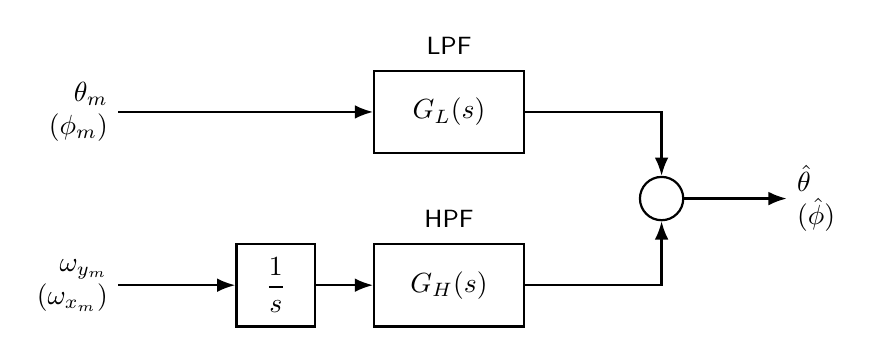
\begin{tikzpicture}[
    >=Latex,
    blk/.style={draw, thick, minimum width=1.9cm, minimum height=1.05cm, align=center},
    sblk/.style={draw, thick, minimum width=1.0cm, minimum height=1.05cm, align=center},
    lbl/.style={font=\small\sffamily, above=2pt},
    sig/.style={->, thick}
  ]
  \node[blk]  (GL)  at (4.2, 1.1)  {$G_L(s)$};
  \node[sblk] (INT) at (2.0,-1.1)  {$\dfrac{1}{s}$};
  \node[blk]  (GH)  at (4.2,-1.1)  {$G_H(s)$};
  \node[draw, thick, circle, minimum size=0.55cm, inner sep=0pt] (sum) at (6.9, 0) {};
  \node[lbl] at (GL.north) {LPF};
  \node[lbl] at (GH.north) {HPF};
  \draw[sig] (0,1.1)  node[left,align=right] {$\theta_m$\\$(\phi_m)$} -- (GL.west);
  \draw[sig] (0,-1.1) node[left,align=right] {$\omega_{y_m}$\\$(\omega_{x_m})$} -- (INT.west);
  \draw[sig] (INT.east) -- (GH.west);
  \draw[sig] (GL.east) -| (sum.north);
  \draw[sig] (GH.east) -| (sum.south);
  \draw[sig] (sum.east) -- ++(1.3,0) node[right,align=left] {$\hat\theta$\\$(\hat\phi)$};
\end{tikzpicture}
\captionof{figure}{Block diagram of the transfer function for pitch estimation; for roll, replace the signals by the ones in parentheses and $L_\theta$ by $L_\phi$.}
\label{fig:complementary-filter}
\end{center}


\end{answer}

% ------------------------------------------------------------ Q4.3 ---
\begin{question}{4.3}{T}
Discuss the impact of changing the tuning parameters Q and R.
\end{question}

\begin{answer}

For the steady state Kalman Filter

\end{answer}

% ------------------------------------------------------------ Q4.4 ---
\begin{question}{4.4}{T+L}
Repeat the Kalman filter design, implementation, and evaluation procedure augmenting
the system with an extra state to capture the bias term on the rate gyro. For that purpose, assume
that
\[ \dot b_y = 0 \]
and
\[ w_{y_m} = q + b_y \]

Suggestion: In the simulation phase, set an artificial bias on the measurement and plot the bias $b_y$ vs. bias estimate $\hat{b}_y$ to guide the tuning of the filter.
\end{question}

\begin{answer}
    \todoanswer
\end{answer}

% ------------------------------------------------------------ Q4.5 ---
\begin{question}{4.5}{T}
Check if the previous filters are complementary. Discuss the advantages and limitations of
this class of filters.
\end{question}

\begin{answer}
    \todoanswer
\end{answer}

% ------------------------------------------------------------ Q4.6 ---
\begin{question}{4.6}{L}
Discuss the results obtained and relate them to the different conditions of operation specified in experiments A to E.
\end{question}

\begin{answer}
    \todoanswer
\end{answer}

% ------------------------------------------------------------ Q4.7 ---
\begin{question}{4.7}{T+L}
Repeat the previous questions for the roll estimation.
\end{question}

\begin{answer}
No separate derivation is needed for roll, since the pitch and roll
channels are decoupled and share the same structure. Every design, transfer
function and result of Questions 4.1--4.6 was therefore obtained for
both angles, using the following correspondence:
\[
  \theta \to \phi, \qquad
  \omega_{y_m} \to \omega_{x_m}, \qquad
  \theta_m \to \phi_m, \qquad
  b_y \to b_x .
\]
The steady-state gains $L$ for roll (Q4.1 and Q4.3), the bias-augmented
filter (Q4.4) and the evaluation on Experiments A to E (Q4.6) are
reported together with the pitch results, in the same tables and figures.
The conclusions on the complementarity of the filters (Q4.5) and on the
effect of $Q$ and $R$ (Q4.3) hold unchanged for roll.
\end{answer}


\end{document}
